\documentclass[12pt, a4paper]{book}

\usepackage{fancyhdr}
\usepackage[left=4cm, right=4cm, top=4cm, bottom=4cm]{geometry}
\usepackage[utf8]{inputenc}
\usepackage[table]{xcolor}
\usepackage{hyperref}
\usepackage{amsmath}
\usepackage{enumitem}
\usepackage{graphicx}
\usepackage{amsfonts}
\usepackage{booktabs}
\usepackage{subcaption}
\usepackage[justification=centering]{caption}
\usepackage{xepersian}

\DeclareMathOperator*{\argmax}{argmax}
\DeclareMathOperator*{\argmin}{argmin}
\newcolumntype{L}{>{$}l<{$}} % math-mode version of "l" column type

\newcommand{\coursetitle}{فهم زبان طبیعی}
\newcommand{\doctitle}{تمرین سوم}
\newcommand{\name}{محمدرضا غفرانی}
\newcommand{\studentno}{400131076}
\newcommand{\todaydate}{\today}

\settextfont{XB Kayhan}
\setlatintextfont{Times Newer Roman}

\pagestyle{fancy}
\rhead{\name}
\lhead{\textbf{\doctitle}}

\begin{document}

\begin{flushleft}
    \name \\
    \studentno \\
    \todaydate
\end{flushleft}

\begin{center}
    \huge
    \textbf{\coursetitle}
    \break
    \large
    \doctitle
\end{center}

% suppress the fancy header on the first page only
\thispagestyle{plain}

\section*{مقدمه}

در این تمرین به مسئله پرسش و پاسخ استخراجی پرداخته‌ایم. هم صورت سوال و هم پاسخ در زبان فارسی بوده است،
البته در بخش سوم تلاش کرده‌ایم تا این مسئله در زبان انگلیسی هم انجام شود.

همانند بسیاری از مسائل حوزه هوش مصنوعی ابتدا لازم است که پیش‌پردازش شود. مجموعه‌داده \lr{PQuAD}
نیاز به پیش‌پردازش خاصی ندارد و صرفا ساختار آن را به نحوی تغییر می‌دهیم که برای ارائه به مدل
ساده‌تر باشد. در این فرمت جدید هر سوال به همراه جواب و متنی که بر اساس آن جواب استخراج شده است
به مدل داده می‌شود. در گام بعدی کلمات مجموعه‌داده به توکن‌ها تبدیل شده و شناسه هر توکن در مدل به آن
نسبت داده می‌شود. همچنین \lr{span} جواب در متن نیز مشخص می‌شود.
قدم بعدی دادن داده‌ها به مدل و گرفتن نتایج است.

به همراه این فایل گزارش سه فایل \lr{convert\_squad\_format\_to\_trainer.py}، \lr{train.py} و \lr{test.py}
وجود دارد. با اجرای فایل \lr{convert\_squad\_format\_to\_trainer.py} فایل‌های آموزش و ارزیابی خوانده شده
و قابل آن‌ها از حالت \lr{json} به \lr{csv} که در مرحله بعد راحت‌تر قابل استفاده است تبدیل می‌شود.
آموزش مدل با اجرای فایل \lr{train.py} انجام می‌شود. برای آموزش مدل از چهارچوب \lr{Huggingface}
استفاده شده است. در هنگام آموزش خطای مدل در داده‌های آموزش و ارزیابی ذخیره می‌شود. با اجرای فایل
\lr{test.py} مدل ذخیره شده ارزیابی می‌شود. برای ارزیابی مدل از نظر \lr{Exact Match} و \lr{F1} ما از
اسکریپت ارائه شده توسط \href{https://huggingface.co/spaces/evaluate-metric/squad_v2}{\lr{Huggingface}} استفاده کرده‌ایم.

\section*{بخش اول}

برای این بخش از مدل‌های ازپیش‌آموزش‌دیده‌ای که در زبان فارسی وجود دارد نظیر مدل‌های
\lr{ParsBERT} و \lr{XLM-RoBERTa} استفاده می‌کنیم. نتایج این آموزش در \autoref{part1_results}
آورده شده است. این مدل‌ها ۵ گام آموزش دیده‌اند و نتایج آورده شده مربوط به بهترین عملکرد آن‌ها در
حین آموزش از نظر خطای آموزش است. با مقایسه‌ دقت‌های حاصل شده با دقت‌های مقاله \lr{PQuAD} مشخص می‌شود
که نتایج ما نسبت به نتایج گزارش شده مقاله بهتر است.

\begin{table}[h]
    \setRL
    \centering
    \caption{نتایج آموزش مدل‌های \underline{ازپیش‌آموزش‌دیده} در مجموعه داده \lr{PQuAD}}
    \label{part1_results}
    \begin{tabular}{c|c|c}
        مدل & \lr{EM} & \lr{F1} \\
        \hline
        \lr{XLM-RoBERTa} & $75.60$ & $87.76$ \\
        \lr{ParsBERT v3} & $68.1$ & $81.69$ \\
    \end{tabular}
\end{table}

در ادامه نتایج عملکرد مدل \lr{XLM-RoBERTa} که نتایج بهتری نسبت به باقی مدل‌ها دارد،
در هر گام آموزش مدل آورده شده است (\autoref{part1_training}). خطای مدل در داده‌های ارزیابی
در گام‌های اول یادگیری رفته‌رفته کم شده است اما پس از مدتی مدل دچار بیش‌برازش شده و
در نتیجه خطای مدل روی داده‌های ارزیابی بد‌تر شده است. در این جا ما نتایج را با استفاده از
مدل ذخیره‌شده در گام ۲۰۰۰ام ارائه کرده‌ایم.

\begin{figure}[h]
    \centering
    \begin{subfigure}{0.45\linewidth}
        \centering
        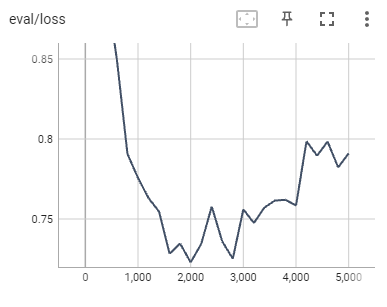
\includegraphics[width=\linewidth]{image/part1/tb/3.png}
    \end{subfigure}
    \hfil
    \begin{subfigure}{0.45\linewidth}
        \centering
        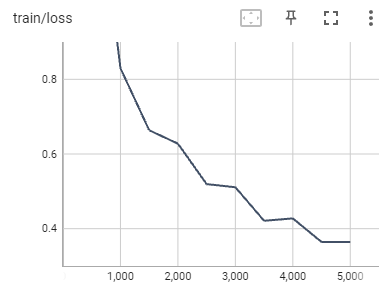
\includegraphics[width=\linewidth]{image/part1/tb/6.png}
    \end{subfigure}
    \caption{عملکرد مدل ازپیش‌آموزش‌دیده \lr{XLM-RoBERTa} در گام‌های مختلف یادگیری}
    \label{part1_training}
\end{figure}

\newpage

در ادامه چند نمونه از پرسش‌وپاسخ انجام شده با استفاده از مدل \lr{XLM-RoBERTa} آورده می‌شود.

\vspace*{0.5cm}

\fbox{%
    \parbox{\textwidth}{
        \textbf{سوال:} کتاب مقدس دین اسلام چیست؟

        \textbf{متن ورودی:} قرآن کتاب مقدس دین اسلام است و در باور مسلمانان سخنان خداست که به صورت وحی از سوی او توسط جبرئیل بر پیامبر اسلام، محمد بن عبدالله، نازل شده‌ است. مسلمانان، قرآن را بزرگترین معجزهٔ محمد و روشن‌ترین دلیل بر پیامبری او می‌دانند. قرآن اصلی‌ترین منبع وحی در اسلام به‌شمار می‌آید و به زبان عربی است. کلمهٔ قرآن در لغت به معنی «قرائت کردن» و «خواندن» است و مسلمانان معمولاً به آن با عناوینی مانند «قرآن کریم» و «قرآن مجید» اشاره می‌کنند. قرآن به ۳۰ جزء تقسیم شده و ۱۱۴ سوره دارد.

        \textbf{پاسخ انتخابی:} قرآن

        \textbf{پاسخ مرجع:} قرآن
    }%
}

\vspace*{0.5cm}

\fbox{%
\parbox{\textwidth}{
    \textbf{سوال:} کتاب فصل الخطاب فی تحریف کتاب رب‌الارباب در چه سالی در ایران چاپ شده‌است؟

    \textbf{متن ورودی:} حسین بن محمد تقی نوری ملقب به خاتم المحدثین در دیباچه کتاب فصل الخطاب فی تحریف کتاب رب‌الارباب می‌نویسد: «این کتابی است لطیف که در اثبات تحریف قرآن، و فضایح اهل جور و عدوان فراهم آورده‌ام، و آن را فصل الخطاب فی تحریف کتاب رب‌الارباب نام نهادم، و بر سه سرآغاز و دو باب قرار دادم». این کتاب در سال ۱۲۹۸ ه‍.ق در ایران چاپ شده‌است. وی در این کتاب برای اثبات ادعای خود بیش از هزار حدیث داستان می‌کند. ولی پس از او دانشمندان شیعه بارها کتاب او را نقد نموده‌اند و احادیث نقل شده در آن کتاب را از باب اختلاف قرائت، برداشت یا مجعول دانسته‌اند.

    \textbf{پاسخ انتخابی:} ۱۲۹۸ ه‍.ق

    \textbf{پاسخ مرجع:} ۱۲۹۸ ه‍.ق
    }%
}

\newpage

\fbox{%
    \parbox{\textwidth}{
        \textbf{سوال:} محبوب‌ترین شاگرد جواد آل محمد چه کسی بود؟

        \textbf{متن ورودی:} محمد تقی با وجود اینکه در خردسالی به امامت رسید و دوران امامتش کوتاه بود، در منابع شیعه و سنی بیش از دویست حدیث در مسائل فقهی، تفسیری، اخلاقی و اعتقادی از او باقی مانده‌است. با این وجود موقعیت علمی وی ظهور و بروز کافی نداشته‌است. جدای از دوران کوتاه امامتش، خردسالی محمد تقی باعث شد سال‌ها طول بکشد تا مورد پذیرش جامعه شیعه واقع شود. دلیل عمده اما تنگنای سیاسی زمانه بود که باعث شد محمد تقی بنا به روایتی تا ده سالگی امامت خود را مخفی نگه دارد. به همین دلیل ارتباط شیعیان با او از طریق نامه‌نگاری صورت می‌گرفت. این نامه‌ها که اغلب نام و نشان کسی که محمد تقی به او نامه می‌نوشته را در خود دارد، بیشتر در جواب سوالات فقهی شیعیان نگاشته شده‌است.

        \textbf{پاسخ انتخابی:} از نظر مدل این سوال با استفاده از این متن قابل پاسخگویی نیست.

        \textbf{پاسخ مرجع}: این سوال با استفاده از این متن قابل پاسخگویی نیست.
    }%
}

\section*{بخش دوم}

در این قسمت نتایج بدون استفاده از پیش‌آموزش مدل‌های فارسی آورده شده است. همان‌طور که مشاهده می‌شود
نتایج نسبت به بخش قبلی افت قابل توجهی داشته‌اند. که این نشان از اهمیت پیش‌آموزش در عملکرد مدل‌های
ترنسفورمری است.

\begin{table}[h]
    \setRL
    \centering
    \caption{نتایج آموزش مدل‌های مختلف \underline{بدون پیش‌آموزش} در مجموعه داده \lr{PQuAD}}
    \label{part2_results}
    \begin{tabular}{c|c|c}
        مدل & \lr{EM} & \lr{F1} \\
        \hline
        \lr{XLM-RoBERTa} & $23.7$ & $28.45$ \\
        \lr{ParsBERT v3} & $25.1$ & $27.48$
    \end{tabular}
\end{table}

در این جا نیز نتایج آموزش ساختار مدل \lr{ParsBERT} را از حالت پایه بررسی می‌کنیم. \autoref{part2_training}
عملکرد مدل در زمان‌های مختلف در هنگام آموزش را نشان می‌دهد. این مدل به دلیل این که ازپیش‌آموزش ندیده است،
بنابراین نه تنها عملکرد ضعیف‌تری از خود نشان می‌دهد بلکه در طی ۵ گام آموزش نیز دچار بیش‌برازش نشده است
و شاید حتی می‌شد که چند گام دیگر را نیز برای آموزش طی کند.

\begin{figure}[h]
    \centering
    \begin{subfigure}{0.45\linewidth}
        \centering
        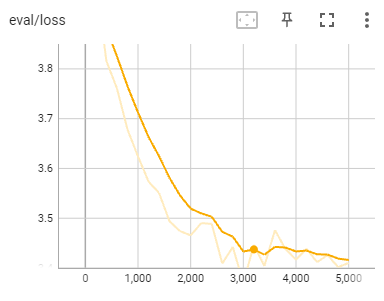
\includegraphics[width=\linewidth]{image/part2/tb/3.png}
    \end{subfigure}
    \hfil
    \begin{subfigure}{0.45\linewidth}
        \centering
        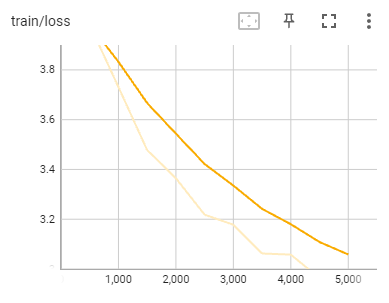
\includegraphics[width=\linewidth]{image/part2/tb/6.png}
    \end{subfigure}
    \caption{عملکرد مدل ازپیش‌آموزش‌دیده \lr{PasrBERT v3} در گام‌های مختلف یادگیری}
    \label{part2_training}
\end{figure}

\newpage

در ادامه نیز چند نمونه از سوال‌ و جواب‌هایی که با مدل انجام داده شده است آورده می‌شود.

\vspace*{0.5cm}

\fbox{%
    \parbox{\textwidth}{
        \textbf{سوال:} کتاب مقدس دین اسلام چیست؟

        \textbf{متن ورودی:} قرآن کتاب مقدس دین اسلام است و در باور مسلمانان سخنان خداست که به صورت وحی از سوی او توسط جبرئیل بر پیامبر اسلام، محمد بن عبدالله، نازل شده‌ است. مسلمانان، قرآن را بزرگترین معجزهٔ محمد و روشن‌ترین دلیل بر پیامبری او می‌دانند. قرآن اصلی‌ترین منبع وحی در اسلام به‌شمار می‌آید و به زبان عربی است. کلمهٔ قرآن در لغت به معنی «قرائت کردن» و «خواندن» است و مسلمانان معمولاً به آن با عناوینی مانند «قرآن کریم» و «قرآن مجید» اشاره می‌کنند. قرآن به ۳۰ جزء تقسیم شده و ۱۱۴ سوره دارد.

        \textbf{پاسخ انتخابی:} از نظر مدل این سوال با استفاده از این متن قابل پاسخگویی نیست.

        \textbf{پاسخ مرجع:} قرآن
    }%
}

\vspace*{0.5cm}

\fbox{%
\parbox{\textwidth}{
    \textbf{سوال:} کتاب فصل الخطاب فی تحریف کتاب رب‌الارباب در چه سالی در ایران چاپ شده‌است؟

    \textbf{متن ورودی:} حسین بن محمد تقی نوری ملقب به خاتم المحدثین در دیباچه کتاب فصل الخطاب فی تحریف کتاب رب‌الارباب می‌نویسد: «این کتابی است لطیف که در اثبات تحریف قرآن، و فضایح اهل جور و عدوان فراهم آورده‌ام، و آن را فصل الخطاب فی تحریف کتاب رب‌الارباب نام نهادم، و بر سه سرآغاز و دو باب قرار دادم». این کتاب در سال ۱۲۹۸ ه‍.ق در ایران چاپ شده‌است. وی در این کتاب برای اثبات ادعای خود بیش از هزار حدیث داستان می‌کند. ولی پس از او دانشمندان شیعه بارها کتاب او را نقد نموده‌اند و احادیث نقل شده در آن کتاب را از باب اختلاف قرائت، برداشت یا مجعول دانسته‌اند.

    \textbf{پاسخ انتخابی:} ۱۲۹۸ ه‍.ق

    \textbf{پاسخ مرجع:} ۱۲۹۸ ه‍.ق
    }%
}

\vspace*{0.5cm}

\fbox{%
    \parbox{\textwidth}{
        \textbf{سوال:} محبوب‌ترین شاگرد جواد آل محمد چه کسی بود؟

        \textbf{متن ورودی:} محمد تقی با وجود اینکه در خردسالی به امامت رسید و دوران امامتش کوتاه بود، در منابع شیعه و سنی بیش از دویست حدیث در مسائل فقهی، تفسیری، اخلاقی و اعتقادی از او باقی مانده‌است. با این وجود موقعیت علمی وی ظهور و بروز کافی نداشته‌است. جدای از دوران کوتاه امامتش، خردسالی محمد تقی باعث شد سال‌ها طول بکشد تا مورد پذیرش جامعه شیعه واقع شود. دلیل عمده اما تنگنای سیاسی زمانه بود که باعث شد محمد تقی بنا به روایتی تا ده سالگی امامت خود را مخفی نگه دارد. به همین دلیل ارتباط شیعیان با او از طریق نامه‌نگاری صورت می‌گرفت. این نامه‌ها که اغلب نام و نشان کسی که محمد تقی به او نامه می‌نوشته را در خود دارد، بیشتر در جواب سوالات فقهی شیعیان نگاشته شده‌است.

        \textbf{پاسخ انتخابی:} از نظر مدل این سوال با استفاده از این متن قابل پاسخگویی نیست.

        \textbf{پاسخ مرجع}: این سوال با استفاده از این متن قابل پاسخگویی نیست.
    }%
}

\section*{بخش سوم}

در این قسمت ما تلاش می‌کنیم مدلی ارائه دهیم که هم بر روی مجموعه داده فارسی و هم بر روی مجموعه داده انگلیسی
قابل استفاده باشد. برای ارائه چنین مدلی از مدل از‌پیش‌آموزش‌دیده \lr{XLM-RoBERTa} استفاده می‌کنیم. علت انتخاب این مدل
نسبت به مدل \lr{ParsBERT} دیدن زبان‌های مختلف در حین پیش‌آموزش مدل است.

نحوه آموزش مدل نیز به این صورت است که ما مجموعه‌های آموزشی \lr{PQuAD} و \lr{SQuAD} را با هم ترکیب کرده و
به مدل می‌دهیم. مدل در هر گام آموزشی بخشی از داده‌های انگلیسی و بخشی از داده‌های فارسی را می‌بیند. در هنگام ارزیابی
نیز یک بار مدل را روی ترکیب مجموعه‌داده‌های \lr{SQuAD} و \lr{PQuAD} ارزیابی می‌کنیم و بار دیگر جداگانه روی هر یک از مجموعه‌ها.
نتایج این آموزش در \autoref{part3_results} آورده شده است. با مقایسه این نتایج با نتایج \autoref{part1_results}
مشاهده می‌کنیم که نتایج روی مجموعه‌داده \lr{PQuAD} اندکی بهتر شده است. علت بهتر شدن نتایج بیشتر شدن
انتظار از مدل و دادن وظایف بیشتر جهت انجام دادن است که باعث شده است مدل تلاش کند بهتر متن ورودی به زبان
فارسی را درک کند.

\begin{table}[h]
    \setRL
    \centering
    \caption{نتایج آموزش مدل‌های مختلف \underline{از‌پیش‌آموزش‌دیده} در مجموعه داده \lr{PQuAD} و \lr{SQuAD}}
    \label{part3_results}
    \begin{tabular}{c|c|c|c|c|c|c}
        & \multicolumn{2}{c|}{\lr{Overal}} & \multicolumn{2}{c|}{\lr{PQuAD}} & \multicolumn{2}{c}{\lr{SQuAD}} \\
        \hline
        مدل              & \lr{EM} & \lr{F1}  & \lr{EM} & \lr{F1} & \lr{EM} & \lr{F1}\\
        \hline
        \lr{XLM-RoBERTa} & $76.93$  & $84.66$ & $76.35$ & $88.36$ & $77.63$ & $80.11$
    \end{tabular}
\end{table}

در ادامه نیز عملکرد مدل \lr{XLM-RoBERTa} در حین آموزش آورده می‌شود (\autoref{part3_training}).
در این جا نیز مشابه بخش اول، عملکرد مدل رفته‌رفته بهتر شده است اما بس از مدتی پدیده بیش‌برازش رخ داده و
خطای مدل روی داده‌های ارزیابی بیشتر شده است. البته همچنان در حالت بیش‌برازش نیز عملکرد مدل از نظر دقت و
بازیابی افت نکرده است.

\begin{figure}[h]
    \centering
    \begin{subfigure}{0.45\linewidth}
        \centering
        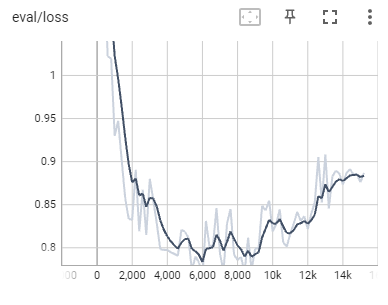
\includegraphics[width=\linewidth]{image/part3/tb/3.png}
    \end{subfigure}
    \hfil
    \begin{subfigure}{0.45\linewidth}
        \centering
        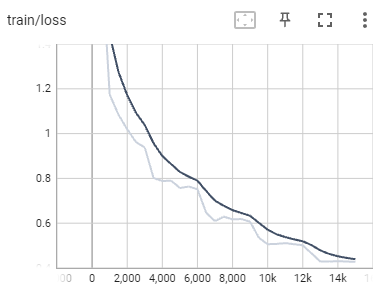
\includegraphics[width=\linewidth]{image/part3/tb/6.png}
    \end{subfigure}
    \caption{خطای مدل ازپیش‌آموزش‌دیده \lr{XLM-RoBERTa} در گام‌های مختلف یادگیری در بخش سوم}
    \label{part3_training}
\end{figure}

\newpage

در ادامه چند نمونه از پرسش‌وپاسخ‌هایی که با مدل انجام شده است آورده می‌شود.

\vspace*{0.5cm}

\fbox{%
    \parbox{\textwidth}{
        \textbf{سوال:} کتاب مقدس دین اسلام چیست؟

        \textbf{متن ورودی:} قرآن کتاب مقدس دین اسلام است و در باور مسلمانان سخنان خداست که به صورت وحی از سوی او توسط جبرئیل بر پیامبر اسلام، محمد بن عبدالله، نازل شده‌ است. مسلمانان، قرآن را بزرگترین معجزهٔ محمد و روشن‌ترین دلیل بر پیامبری او می‌دانند. قرآن اصلی‌ترین منبع وحی در اسلام به‌شمار می‌آید و به زبان عربی است. کلمهٔ قرآن در لغت به معنی «قرائت کردن» و «خواندن» است و مسلمانان معمولاً به آن با عناوینی مانند «قرآن کریم» و «قرآن مجید» اشاره می‌کنند. قرآن به ۳۰ جزء تقسیم شده و ۱۱۴ سوره دارد.

        \textbf{پاسخ انتخابی:} قرآن

        \textbf{پاسخ مرجع:} قرآن
    }%
}

\vspace*{0.5cm}

\fbox{%
    \parbox{\textwidth}{
        \textbf{سوال:} کتاب فصل الخطاب فی تحریف کتاب رب‌الارباب در چه سالی در ایران چاپ شده‌است؟

        \textbf{متن ورودی:} حسین بن محمد تقی نوری ملقب به خاتم المحدثین در دیباچه کتاب فصل الخطاب فی تحریف کتاب رب‌الارباب می‌نویسد: «این کتابی است لطیف که در اثبات تحریف قرآن، و فضایح اهل جور و عدوان فراهم آورده‌ام، و آن را فصل الخطاب فی تحریف کتاب رب‌الارباب نام نهادم، و بر سه سرآغاز و دو باب قرار دادم». این کتاب در سال ۱۲۹۸ ه‍.ق در ایران چاپ شده‌است. وی در این کتاب برای اثبات ادعای خود بیش از هزار حدیث داستان می‌کند. ولی پس از او دانشمندان شیعه بارها کتاب او را نقد نموده‌اند و احادیث نقل شده در آن کتاب را از باب اختلاف قرائت، برداشت یا مجعول دانسته‌اند.

        \textbf{پاسخ انتخابی:} ۱۲۹۸ ه‍.ق

        \textbf{پاسخ مرجع:} ۱۲۹۸ ه‍.ق
    }%
}

\vspace*{0.5cm}

\fbox{%
    \parbox{\textwidth}{
        \textbf{سوال:} محبوب‌ترین شاگرد جواد آل محمد چه کسی بود؟

        \textbf{متن ورودی:} محمد تقی با وجود اینکه در خردسالی به امامت رسید و دوران امامتش کوتاه بود، در منابع شیعه و سنی بیش از دویست حدیث در مسائل فقهی، تفسیری، اخلاقی و اعتقادی از او باقی مانده‌است. با این وجود موقعیت علمی وی ظهور و بروز کافی نداشته‌است. جدای از دوران کوتاه امامتش، خردسالی محمد تقی باعث شد سال‌ها طول بکشد تا مورد پذیرش جامعه شیعه واقع شود. دلیل عمده اما تنگنای سیاسی زمانه بود که باعث شد محمد تقی بنا به روایتی تا ده سالگی امامت خود را مخفی نگه دارد. به همین دلیل ارتباط شیعیان با او از طریق نامه‌نگاری صورت می‌گرفت. این نامه‌ها که اغلب نام و نشان کسی که محمد تقی به او نامه می‌نوشته را در خود دارد، بیشتر در جواب سوالات فقهی شیعیان نگاشته شده‌است.

        \textbf{پاسخ انتخابی:} از نظر مدل این سوال با استفاده از این متن قابل پاسخگویی نیست.

        \textbf{پاسخ مرجع}: این سوال با استفاده از این متن قابل پاسخگویی نیست.
    }%
}

\newpage


\fbox{%
\parbox{\textwidth}{
    \textbf{سوال:} \lr{What do most online pharmacies do?}

    \textbf{متن ورودی:} \lr{While most Internet pharmacies sell prescription drugs and require a valid prescription, some Internet pharmacies sell prescription drugs without requiring a prescription. Many customers order drugs from such pharmacies to avoid the \"inconvenience\" of visiting a doctor or to obtain medications which their doctors were unwilling to prescribe. However, this practice has been criticized as potentially dangerous, especially by those who feel that only doctors can reliably assess contraindications, risk/benefit ratios, and an individual's overall suitability for use of a medication. There also have been reports of such pharmacies dispensing substandard products.}

    \textbf{پاسخ انتخابی:} \lr{sell prescription drugs}

    \textbf{پاسخ مرجع:} \lr{sell prescription drugs}
    }%
}

\vspace*{0.5cm}

\fbox{%
    \parbox{\textwidth}{
        \textbf{سوال:} \lr{What is the minimum distance between a patient's home and the nearest pharmacy that allows a physician in Austria to give out medicine?}

        \textbf{متن ورودی:} \lr{In some rural areas in the United Kingdom, there are dispensing physicians who are allowed to both prescribe and dispense prescription-only medicines to their patients from within their practices. The law requires that the GP practice be located in a designated rural area and that there is also a specified, minimum distance (currently 1.6 kilometres) between a patient's home and the nearest retail pharmacy. This law also exists in Austria for general physicians if the nearest pharmacy is more than 4 kilometers away, or where none is registered in the city.}

        \textbf{پاسخ انتخابی:} از نظر مدل این سوال با استفاده از این متن قابل پاسخگویی نیست.

        \textbf{پاسخ مرجع:} \lr{more than 4 kilometers}
    }%
}

\newpage

\fbox{%
    \parbox{\textwidth}{
        \textbf{سوال:} \lr{What kind of division of power did Kublai's government never have?}

        \textbf{متن ورودی:} \lr{The system of bureaucracy created by Kublai Khan reflected various cultures in the empire, including that of the Han Chinese, Khitans, Jurchens, Mongols, and Tibetan Buddhists. While the official terminology of the institutions may indicate the government structure was almost purely that of native Chinese dynasties, the Yuan bureaucracy actually consisted of a mix of elements from different cultures. The Chinese-style elements of the bureaucracy mainly came from the native Tang, Song, as well as Khitan Liao and Jurchen Jin dynasties. Chinese advisers such as Liu Bingzhong and Yao Shu gave strong influence to Kublai's early court, and the central government administration was established within the first decade of Kublai's reign. This government adopted the traditional Chinese tripartite division of authority among civil, military, and censorial offices, including the Central Secretariat (Zhongshu Sheng) to manage civil affairs, the Privy Council (Chinese: 樞密院) to manage military affairs, and the Censorate to conduct internal surveillance and inspection. The actual functions of both central and local government institutions, however, showed a major overlap between the civil and military jurisdictions, due to the Mongol traditional reliance on military institutions and offices as the core of governance. Nevertheless, such a civilian bureaucracy, with the Central Secretariat as the top institution that was (directly or indirectly) responsible for most other governmental agencies (such as the traditional Chinese-style Six Ministries), was created in China. At various times another central government institution called the Department of State Affairs (Shangshu Sheng) that mainly dealt with finance was established (such as during the reign of Külüg Khan or Emperor Wuzong), but was usually abandoned shortly afterwards.}

        \textbf{پاسخ انتخابی:} از نظر مدل این سوال با استفاده از این متن قابل پاسخگویی نیست.

        \textbf{پاسخ مرجع:} این سوال با استفاده از این متن قابل پاسخگویی نیست.
    }%
}

\section*{جمع‌بندی و نتیجه‌گیری}

در این تمرین ما مدل‌های مختلفی را برای وظیفه پرسش‌وپاسخ در زبان فارسی را بررسی کردیم.
مقایسه نتایج در بخش‌های اول و دوم اهمیت پیش‌آموزش را در عملکرد مدل‌های ترنسفورمری
نشان می‌دهد. در بخش سوم نیز با اضافه شدن مجموعه‌داده انگلیسی به مجموعه‌دادگان آموزش و ارزیابی عملکرد مدل نسبت
به نتایج بخش اول اندکی بهبود یافت.

\end{document}